\chapter{Part I(c) - ISA Memory and Addressing Modes - W 2.1}

\section{Memory}
\textit{Memory is a really important component of a computing system, we store our programs in it, we store our data in it, and it's through memory that we receive and send data.} \\ \vspace*{5px}
\textbf{Though memory is very useful it has three main drawbacks:} \\ \vspace*{5px}
\begin{itemize}
    \item[-] It's \textbf{slow} $\rightarrow$ Caches 
    \item[-] It's \textbf{finite} $\rightarrow$ Virtual Memory
    \item[-] It can make an ISA \textbf{too complex} $\rightarrow$ Pipelining
\end{itemize}
\textit{no worries we'll cover each one of these in this chapter.}

\subsection{Address and Data}
\textit{Data in Memory can be accessed by an adress, meaning i's a \textit{Random Access} (it can access a memory value without going through the preceding ones).} \\ \vspace*{5px}
\textit{Professor Remark: "There's not anything random about this memory, we'd better call it and abitrary access memory. (!not and official  name)"} \\ \vspace*{5px}
\vspace*{5px}
\begin{minipage}[htp]{0.45\textwidth}
\begin{center}
    \begin{tabular}{|c|c|}
    \hline
    \textbf{Address} & \textbf{Value} \\
    \hline
    \texttt{0} & 12 \\ 
    \hline
    \texttt{1} & 6 \\ 
    \hline
    \texttt{2} & 4 \\ 
    \hline
    \texttt{3} & 1 \\ 
    \hline
    \texttt{4} & 0 \\ 
    \hline
    \texttt{5} & 3 \\ 
    \hline
    \texttt{6} & 1 \\ 
    \hline
    \texttt{7} & 13 \\ 
    \hline
    \texttt{8} & 15 \\ 
    \hline
    \texttt{9} & 9 \\ 
    \hline
    \texttt{10} & 3 \\ 
    \hline
    \texttt{11} & 5 \\ 
    \hline
    \texttt{12} & 0 \\ 
    \hline
    \texttt{13} & 0 \\ 
    \hline
    \texttt{14} & 0 \\ 
    \hline
    \texttt{15} & 0 \\ 
    \hline
    \end{tabular}
\end{center}
\end{minipage}
\hfill
\vline
\hfill
\begin{minipage}[htp]{0.45\textwidth}
\begin{center}
    \begin{tabular}{|c|c|}
    \hline
    \textbf{Write} & \textbf{Read} \\ 
    \hline
    \texttt{\textbf{Memory[5] = 3}} & \texttt{Memory[5]?} \\ 
    \hline
    \end{tabular}
\end{center}
\end{minipage}

\section{Many Types of Memories}
We may distinguish between different types of memories based on their \textbf{technology}, such as SRAM, DRAM, EPROM, and Flash, and their \textbf{capabilities}, including \textbf{speed}, \textbf{capacity}, \textbf{density}, \textbf{writability} (whether they are writable, permanent, or reprogrammable), as well as their \textbf{size}, \textbf{volatility}, and \textbf{cost}. \\ \vspace*{5px}
\subsection{Functional Taxonomy of Memories}
\begin{center} 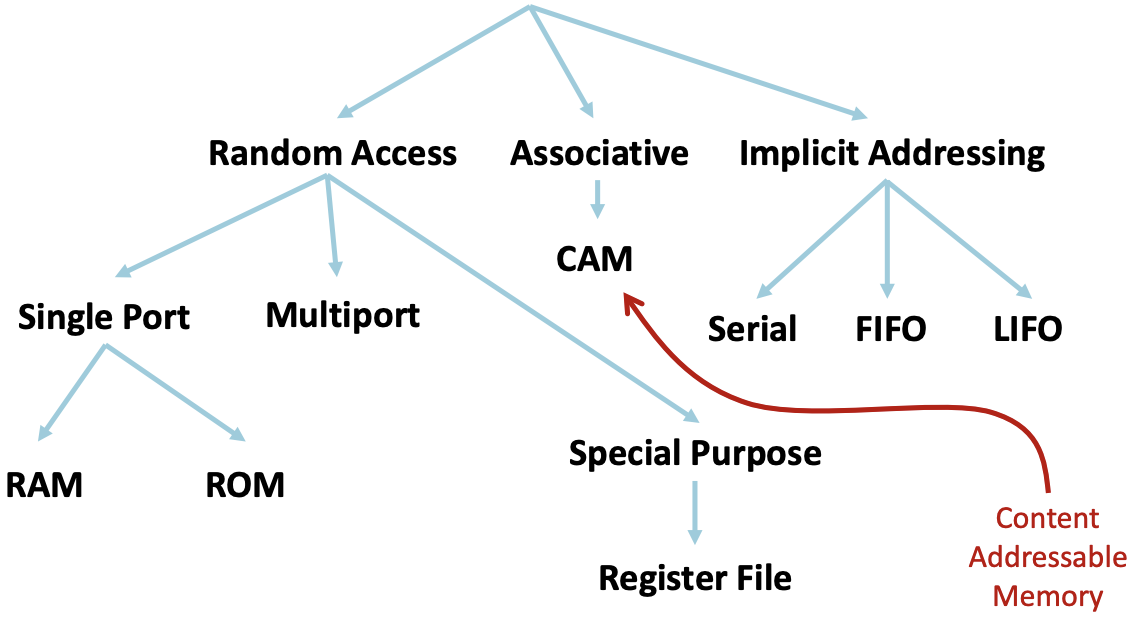
\includegraphics[width=0.45\textwidth]{chapters/chapter1c/images/funct_tax.png} \end{center}
\begin{itemize}
    \item[] \textbf{Multiport} memory allows simultaneous access by multiple processors, while \textbf{single-port} memory supports only one at a time.
    \item[] \textbf{Non-Random Access memories}
    \begin{itemize}
        \item \textbf{Adsociative} memories enable fast data retrieval by content rather than address, making it useful for cache memory, pattern recognition, and efficient lookups in large datasets.
        \item In \textbf{Implicit addressing} the address of the data to be operated on is inferred directly by the operation code (opcode), without explicitly specifying the address in the instruction.
    \end{itemize}
\end{itemize}


\subsection{Taxonomy of Random Access Memories}
\begin{center}
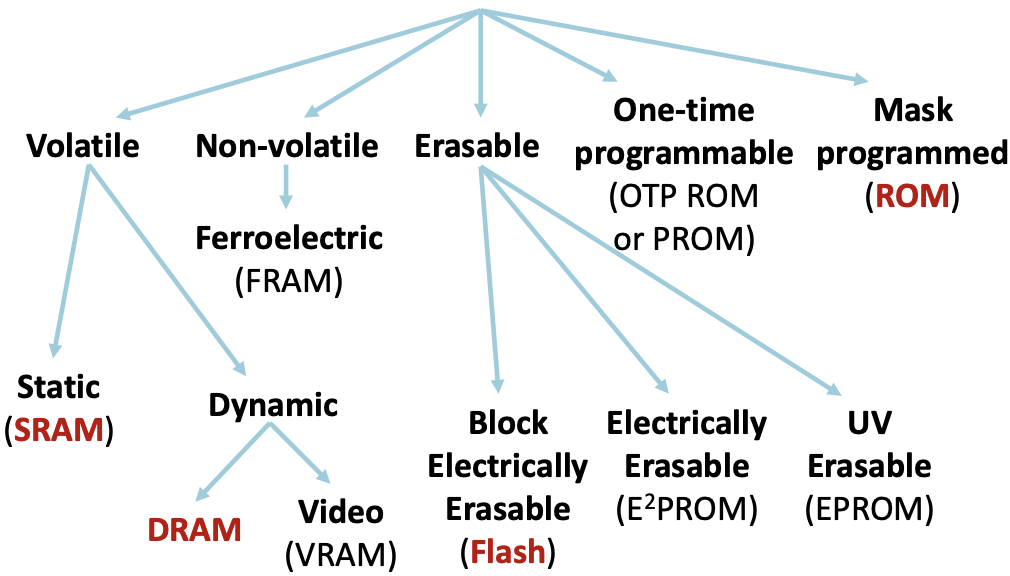
\includegraphics[width=0.45\textwidth]{chapters/chapter1c/images/ram_tax.png}
\end{center}
\newpage
\subsection{Basic Structure}
\textit{Remember, a Data Flip Flop, stores a 1 bit value by updating the output value to the input value at the rising edge of the clock signal.} \\ \vspace*{5px}
\begin{minipage}[htp]{0.35\textwidth} 
\begin{center}
    \begin{tabular}{|c|c|}
        \hline
        \textbf{Address} & \textbf{Value} \\ 
        \hline
        \texttt{0} & 12 \\ 
        \hline
        \texttt{1} & 6 \\ 
        \hline
        \texttt{2} & 4 \\ 
        \hline
        \texttt{3} & 1 \\ 
        \hline
        \texttt{4} & 0 \\ 
        \hline
        \texttt{5} & 3 \\ 
        \hline
        \texttt{6} & 1 \\ 
        \hline
        \texttt{7} & 13 \\ 
        \hline
        \texttt{8} & 15 \\ 
        \hline
        \texttt{9} & 9 \\ 
        \hline
        \texttt{10} & 3 \\ 
        \hline
        \texttt{11} & 5 \\ 
        \hline
        \texttt{12} & 0 \\ 
        \hline
        \texttt{13} & 0 \\ 
        \hline
        \texttt{14} & 0 \\ 
        \hline
        \texttt{15} & 0 \\ 
        \hline
        \end{tabular}
\end{center}
\end{minipage}
\hfill
\vline
\hfill
\begin{minipage}[htp]{0.35\textwidth}
\textbf{16 x 4 Memory Cells (~Special DFFs (Data Flip-Flops))} \\
\begin{center}
    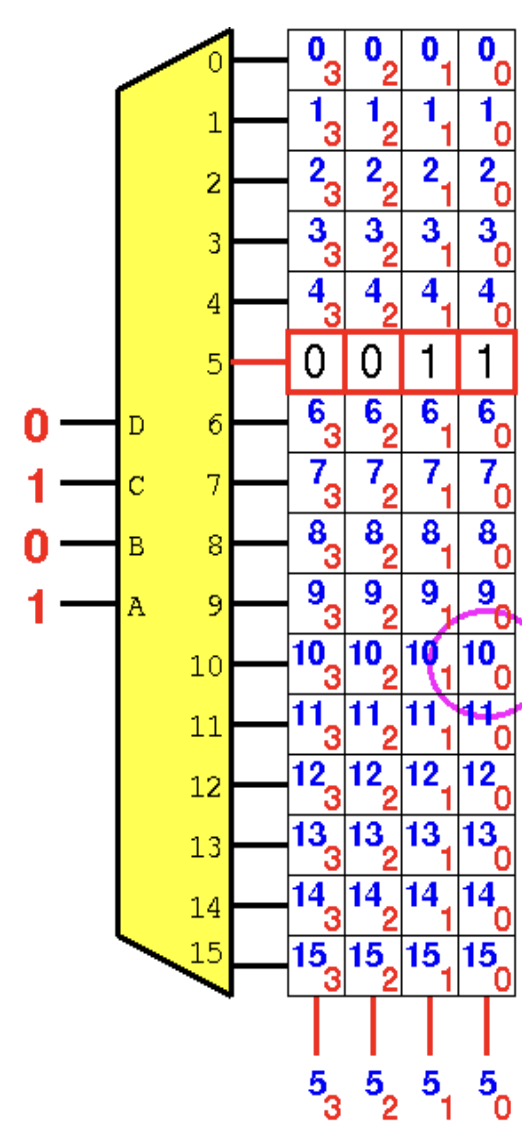
\includegraphics[width=0.45\textwidth]{chapters/chapter1c/images/structure.png}
\end{center}
\end{minipage} \\
\vfill
\begin{minipage}[htp]{0.45\textwidth}   
    \subsection{Write Operations}
    \textit{The D is connected to the Data outside of the system and at the risiing edge it updates the value of the DFF.} \textbf{The AND gate ensures that the write signal is high when the clock signal is high.} \\ \vspace*{5px}
    \begin{center}
        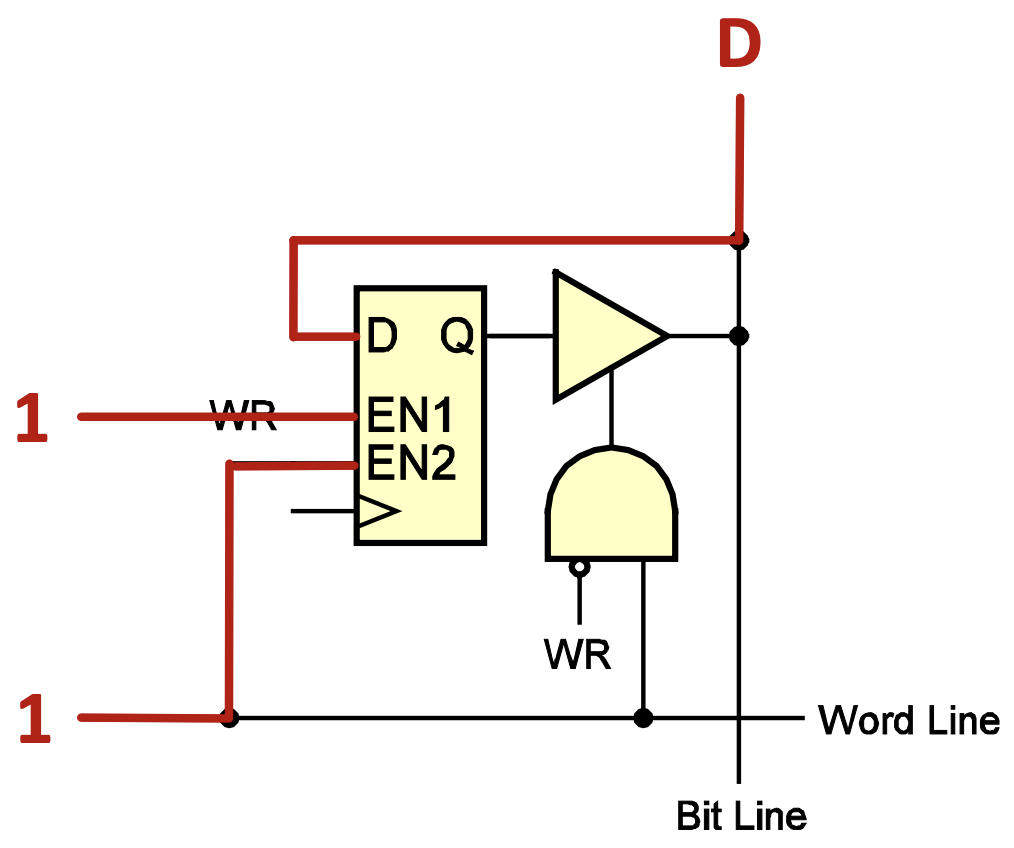
\includegraphics[width=0.45\textwidth]{chapters/chapter1c/images/write.png}
    \end{center}
\end{minipage}
\hfill  
\vline
\hfill
\begin{minipage}[htp]{0.45\textwidth}
    \subsection{Read Operations}
    \textit{D is still connected to the Data, remember the tri-state driver is active when it's enable signal is active (so when the wr is off and the operation signal is sent.).} \\ \vspace*{5px}
    \begin{center}
        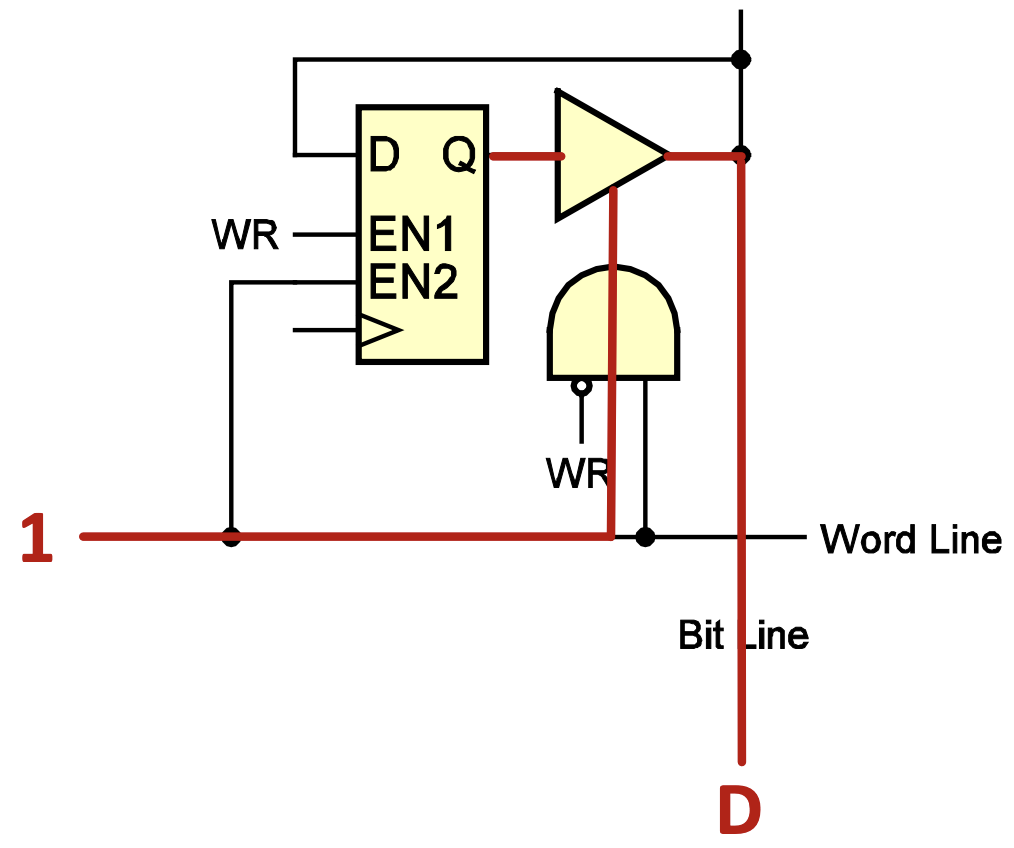
\includegraphics[width=0.45\textwidth]{chapters/chapter1c/images/read.png}
    \end{center}
\end{minipage}

\vspace*{5px}
\subsection{Practical SRAMs}
\textbf{DISCLAIMER !!: Combinational loops are prohibited as they can lead to unstable behavior, unpredictable timing, simulation and synthesis issues, excessive power consumption, and lack of a defined reset state, making them unsuitable for reliable digital circuit design.} \\ \vspace*{5px}
\textit{While the type of memory we've juste seen is small, and very fast, SRAM memories uses 6 transitors per cell (less than the previous design). We've also seen (in Taxonomy) that SRAM is \textbf{static} meaning it doesn't require periodic refresh.} \\ \vspace*{5px}
\begin{minipage}[htp]{0.45\textwidth} 
    \begin{center}
        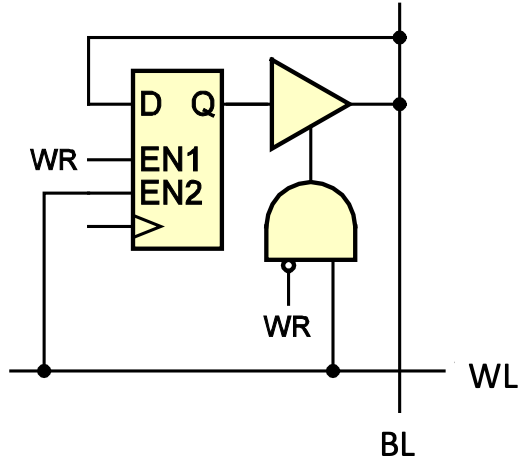
\includegraphics[width=0.55\textwidth]{chapters/chapter1c/images/ram.png}
    \end{center}
    \end{minipage}
    \hfill
    \vline
    \hfill
    \begin{minipage}[htp]{0.45\textwidth}
    \begin{center}
        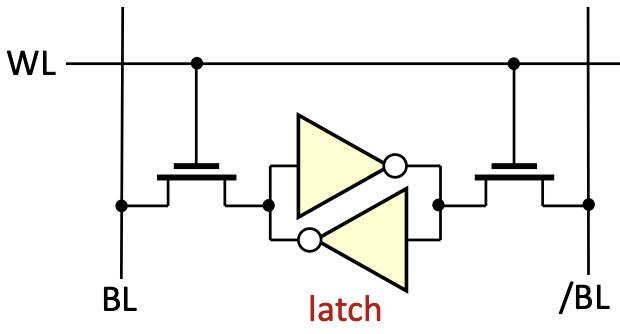
\includegraphics[width=0.55\textwidth]{chapters/chapter1c/images/sram.png}
    \end{center}
    \end{minipage}

\subsection{DRAMs}
\textit{Dynamic RAMS(DRAMs) are the densest and cheapest type of RAM memory, it stores information as charge in small capacitors. This makes the DRAM need periodic refresh otherwise the charge might leak off (~60ms) the capacitor due to parasitic resistances and the information lost} \\ \vspace*{5px}

\begin{minipage}[htp]{0.45\textwidth}
    \textbf{Refresh means, we come back before the end of a charge (~60ms) and we rewrite the value, if there is still some charge, we add charge, if there's no charge and we keep as is.} \\ \vspace*{5px}
    \textit{Personal Remark: Dynamic = Bad, data dissapears and needs refresh}
\end{minipage}
\hfill
\vline  
\hfill
\begin{minipage}[htp]{0.45\textwidth}
    \begin{center}
        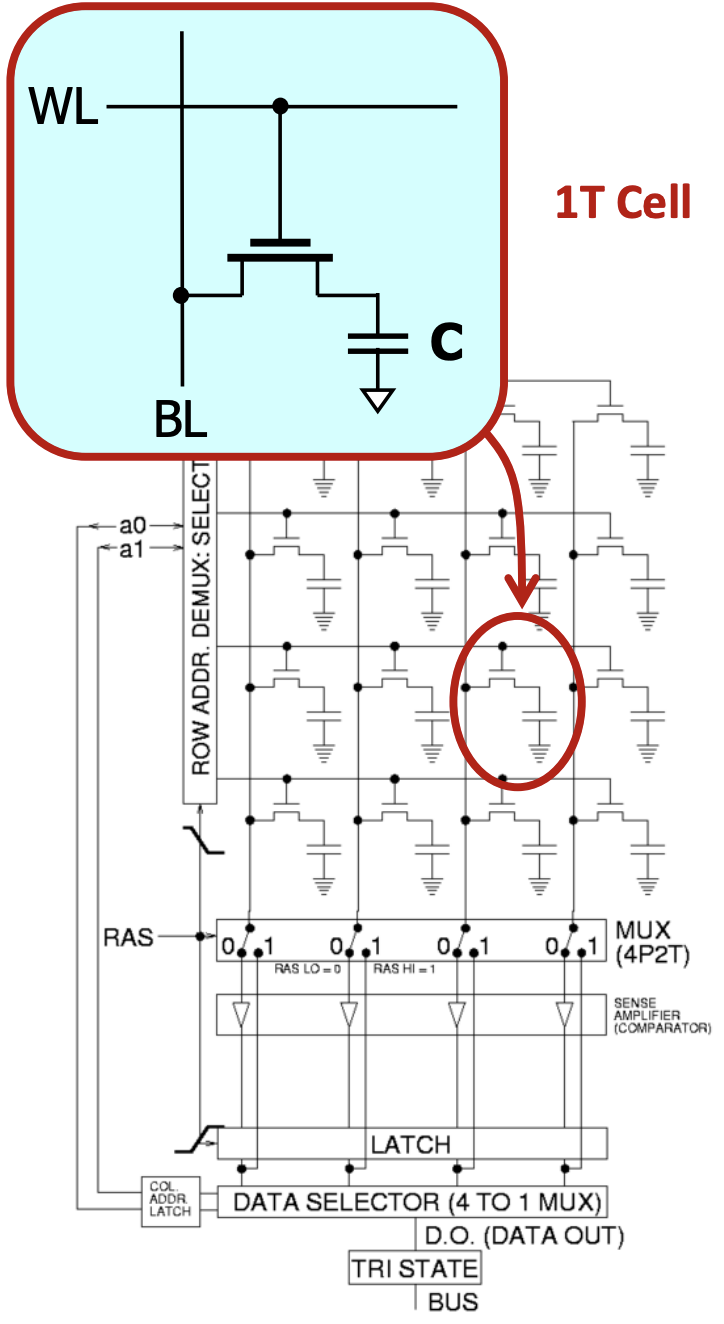
\includegraphics[width=0.5\textwidth]{chapters/chapter1c/images/dram.png}  
    \end{center}
\end{minipage}

\subsection{Ideal Random Access Memory}
\textit{A memory array uses an \(n\)-to-\(2^n\) decoder to select a word line based on the input address, enabling data to be read or written through the bit lines.}
\begin{center}
    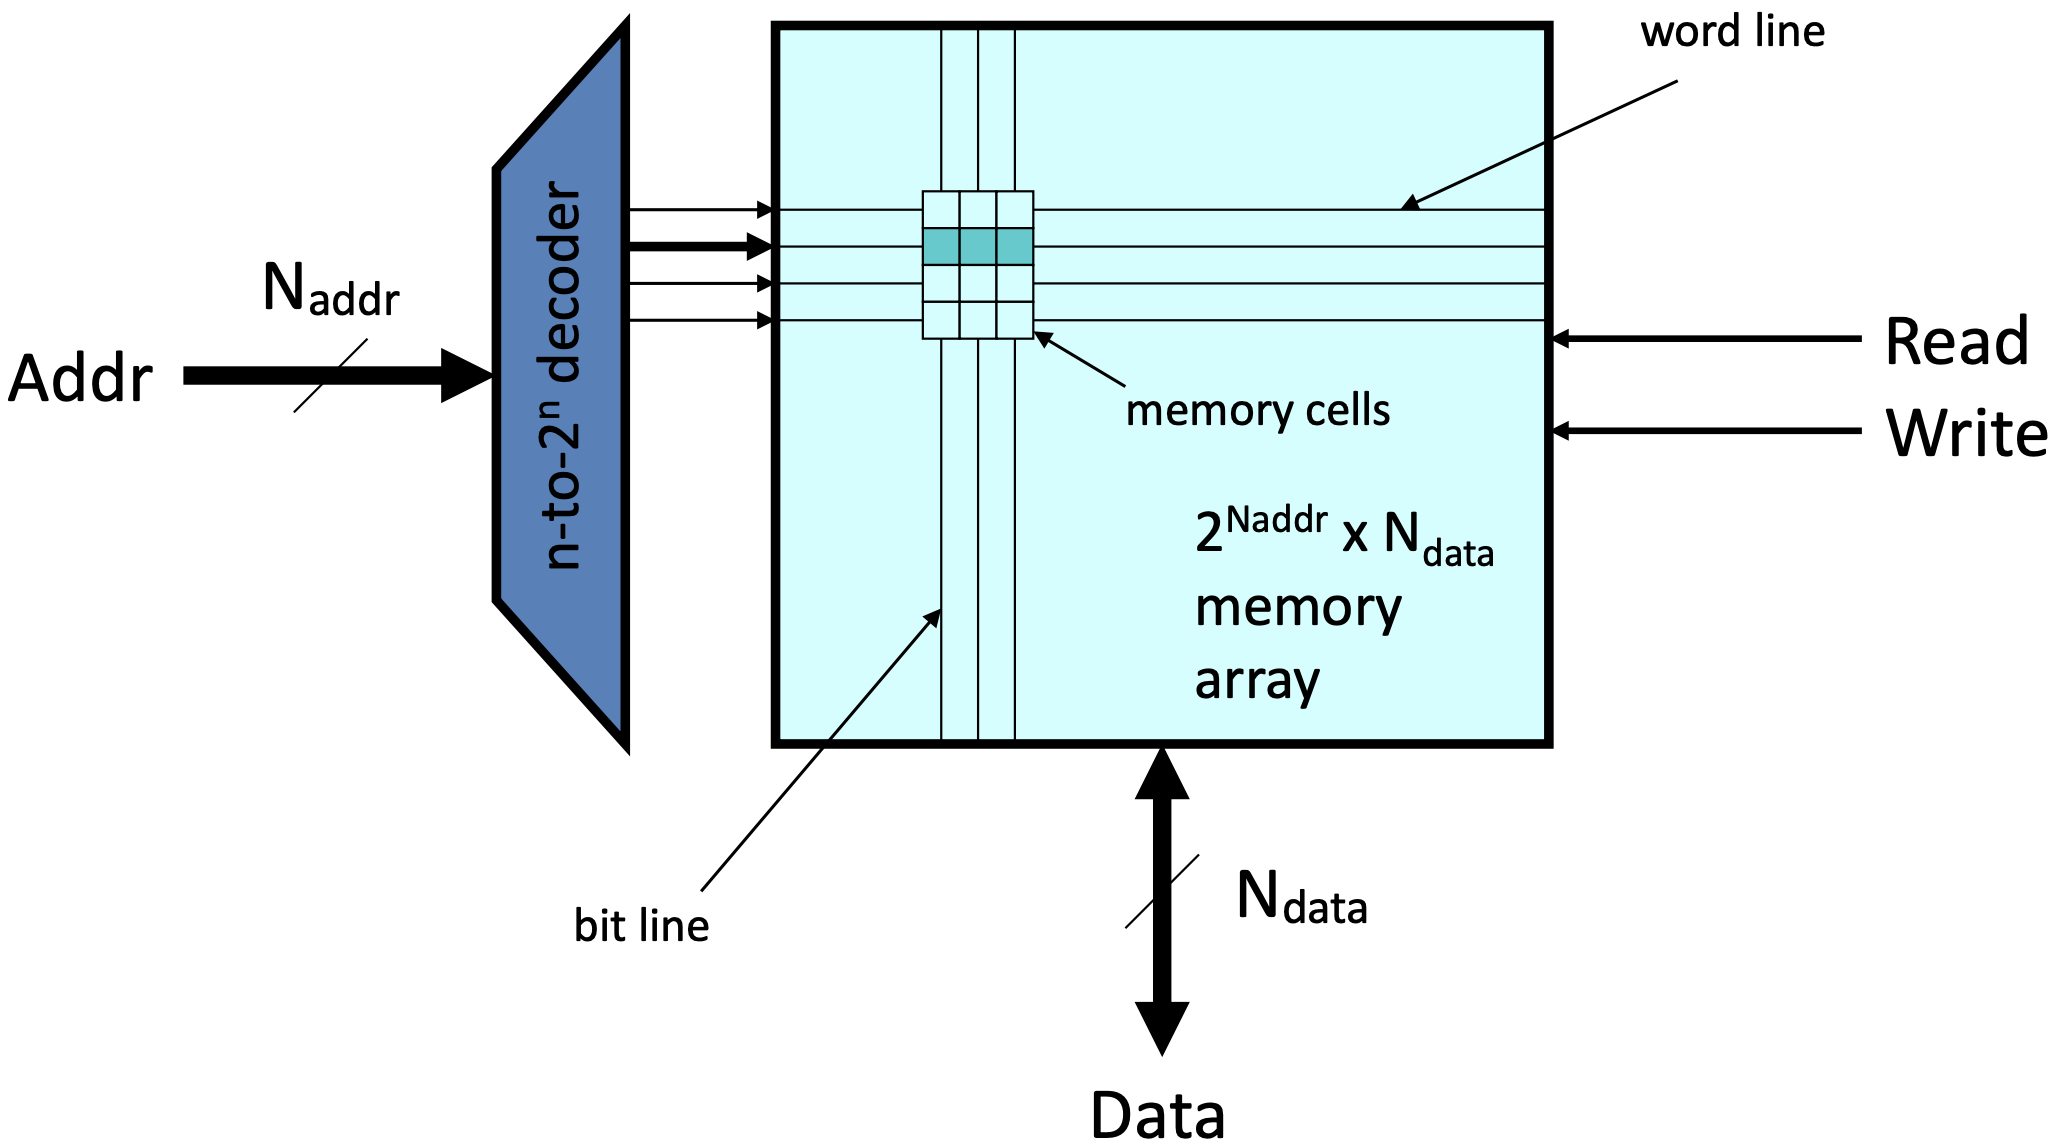
\includegraphics[width=0.45\textwidth]{chapters/chapter1c/images/ideal_ram.png}
\end{center}
\subsection{Physical Organisation }
\begin{center}
    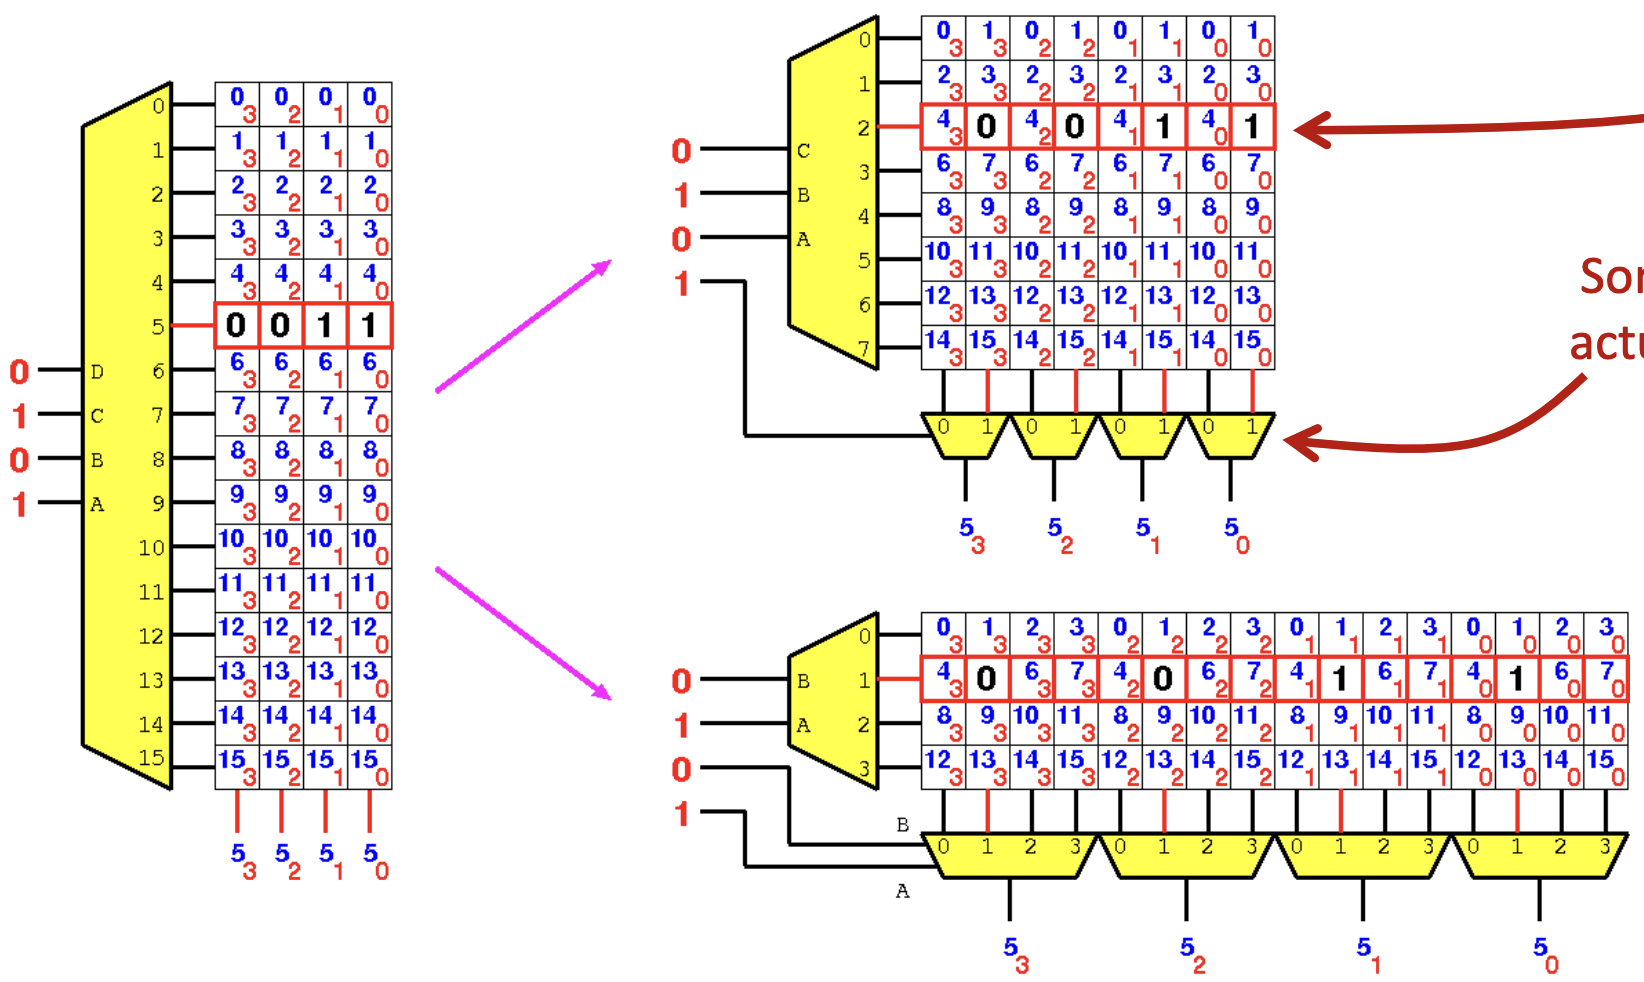
\includegraphics[width=0.45\textwidth]{chapters/chapter1c/images/organisation.png}
\end{center}
\textit{Out of all physical organizations, the squared one is the best one as it has the best performance. This layout facilitates faster access times and simplified wiring, resulting in improved computational efficiency and system scalability.}
\subsection{Realistic ROM Array}
\textit{ROMs are Read-Only Memories, they are used to store the program of the computer, they are non-volatile and can't be written to.} \\ \vspace*{5px}
\begin{center}
    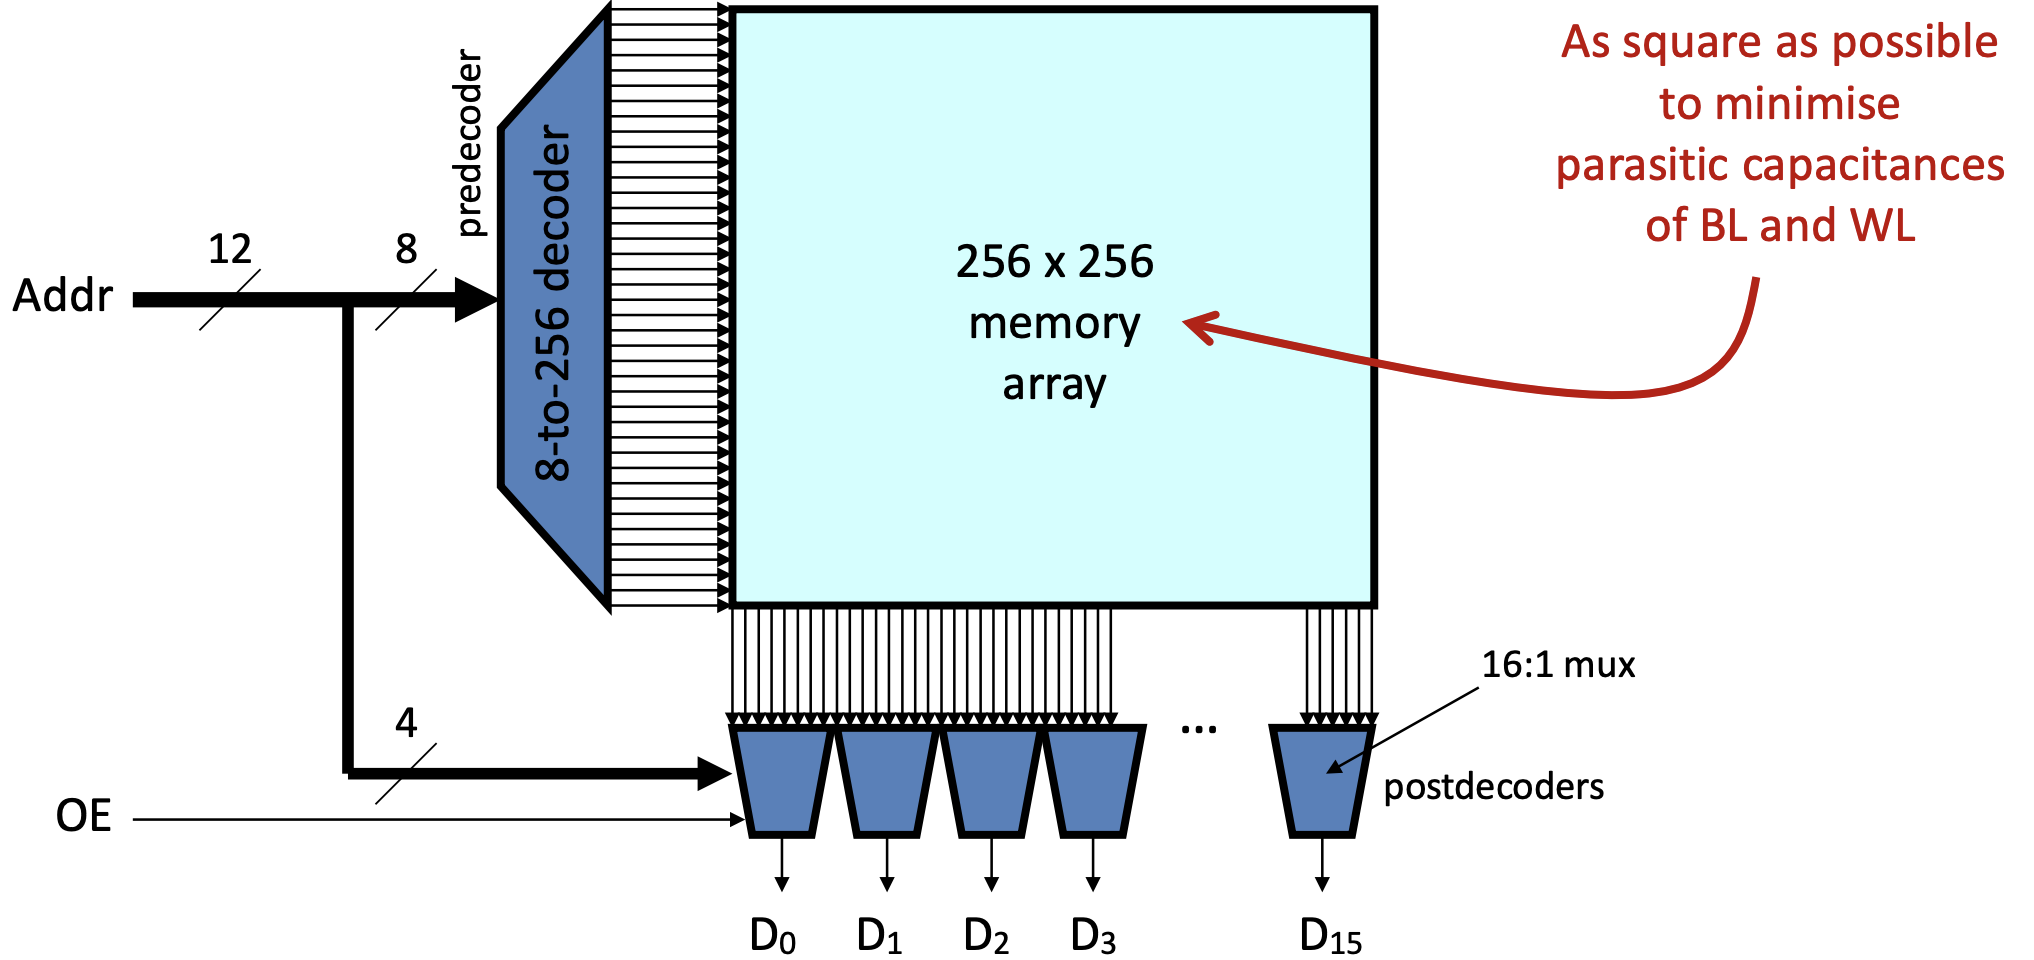
\includegraphics[width=0.45\textwidth]{chapters/chapter1c/images/rom.png}
\end{center}

\subsection{Static Ram Typical Interface}
\textit{This a typical interface of a SRAM, it has a 16-bit data input/output, a 16-bit address input, a write enable signal, and a circuit select signal.}
\begin{center}
    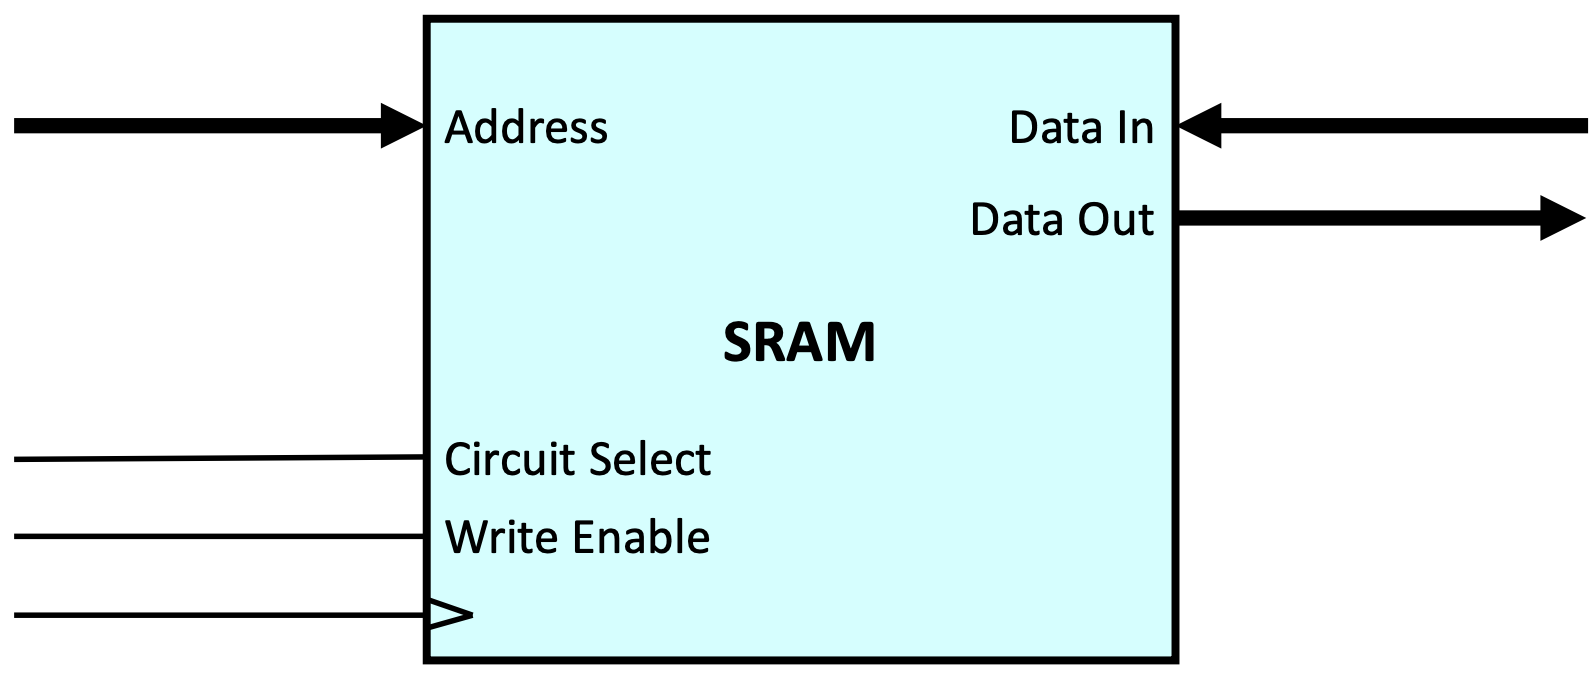
\includegraphics[width=0.45\textwidth]{chapters/chapter1c/images/sram_interface.png}
\end{center}

\section{Typical Asynchronous SRAM Read Cycle}
\textit{The read cycle of an asynchronous SRAM is initiated by the address input, which is decoded to select the word line, enabling the data to be read from the memory array and output to the data bus.} \\ \vspace*{5px}
\textit{Here, Tcyc is the cycle time, Tacc is the access time, and Ten is the enable time.}

\begin{minipage}[htp]{0.45\textwidth}
    \begin{center}
        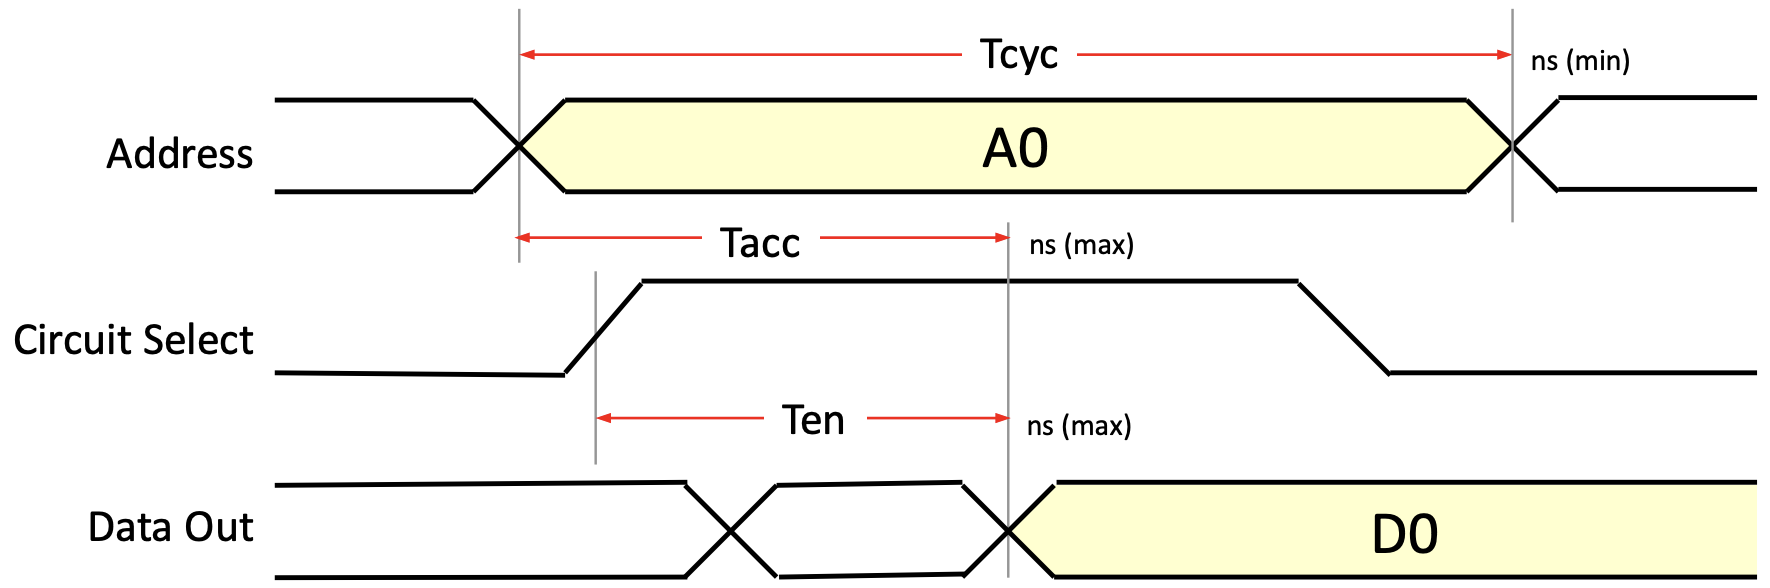
\includegraphics[width=0.45\textwidth]{chapters/chapter1c/images/sram_read.png}
    \end{center}
\end{minipage}
\hfill
\vline
\hfill
\begin{minipage}[htp]{0.45\textwidth}
    \begin{center}
        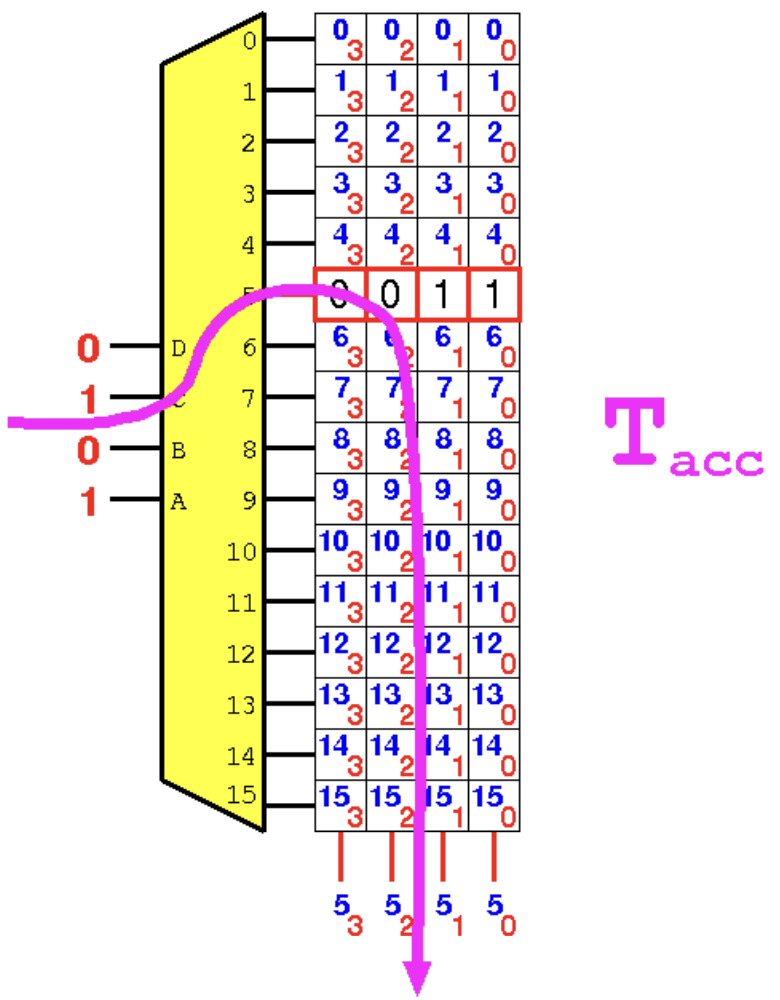
\includegraphics[width=0.45\textwidth]{chapters/chapter1c/images/sram_read2.png}
    \end{center}
\end{minipage}  

\subsubsection{Read Cycle}
\textit{Latency} defined as the number of cycles between the address asserted and data available \\ \vspace*{5px}
\begin{center}
    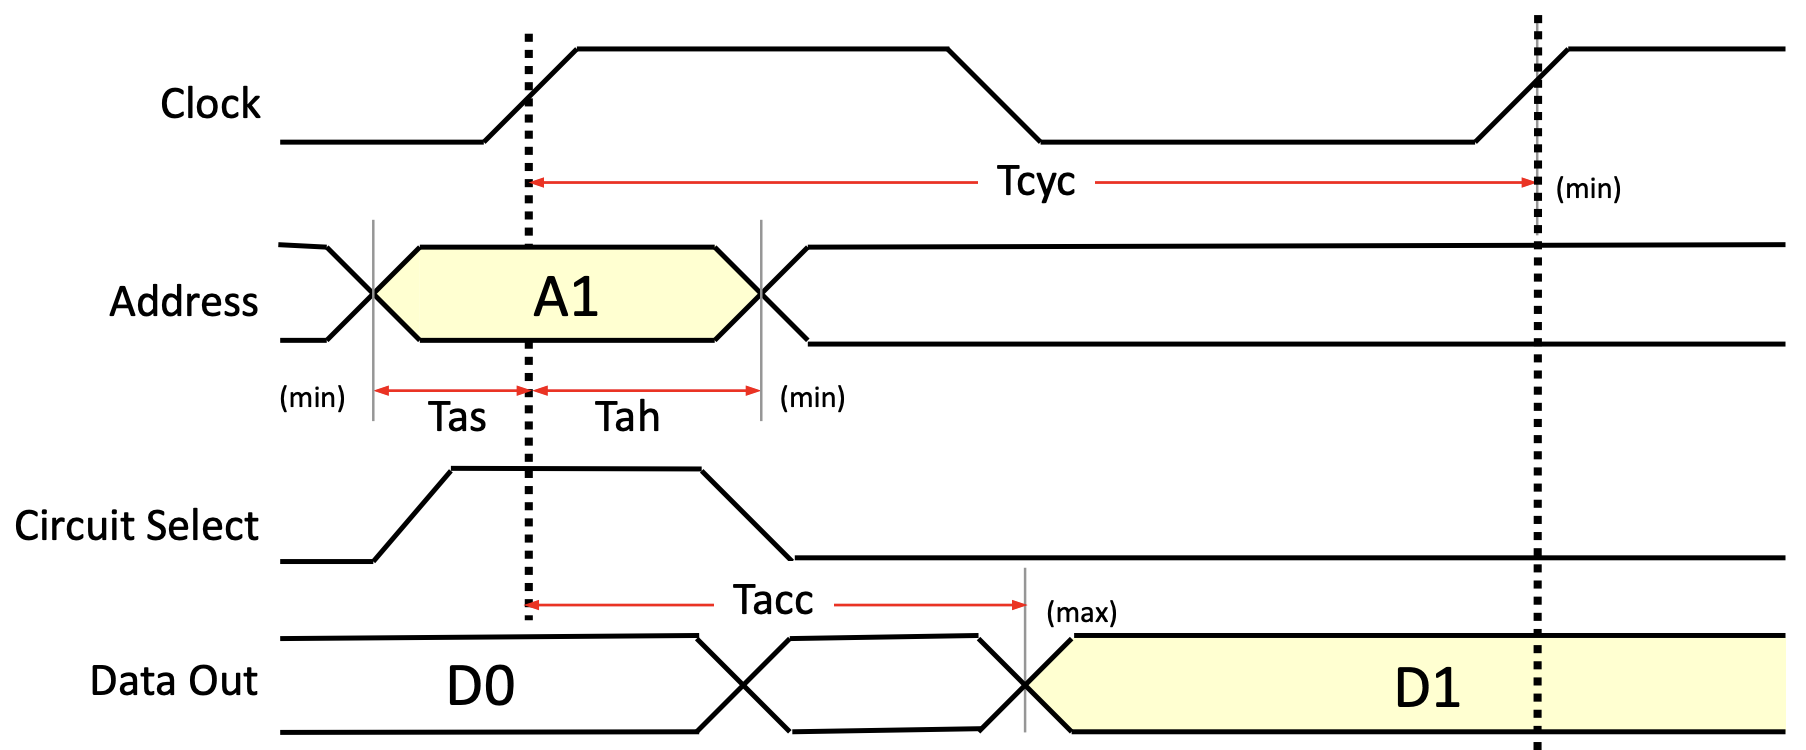
\includegraphics[width=0.45\textwidth]{chapters/chapter1c/images/read_cycle.png}
\end{center}
\subsubsection{Write Cycle}
\textit{Writes on the edge of the clock signal, as a DFF} \\ \vspace*{5px}
\begin{center}
    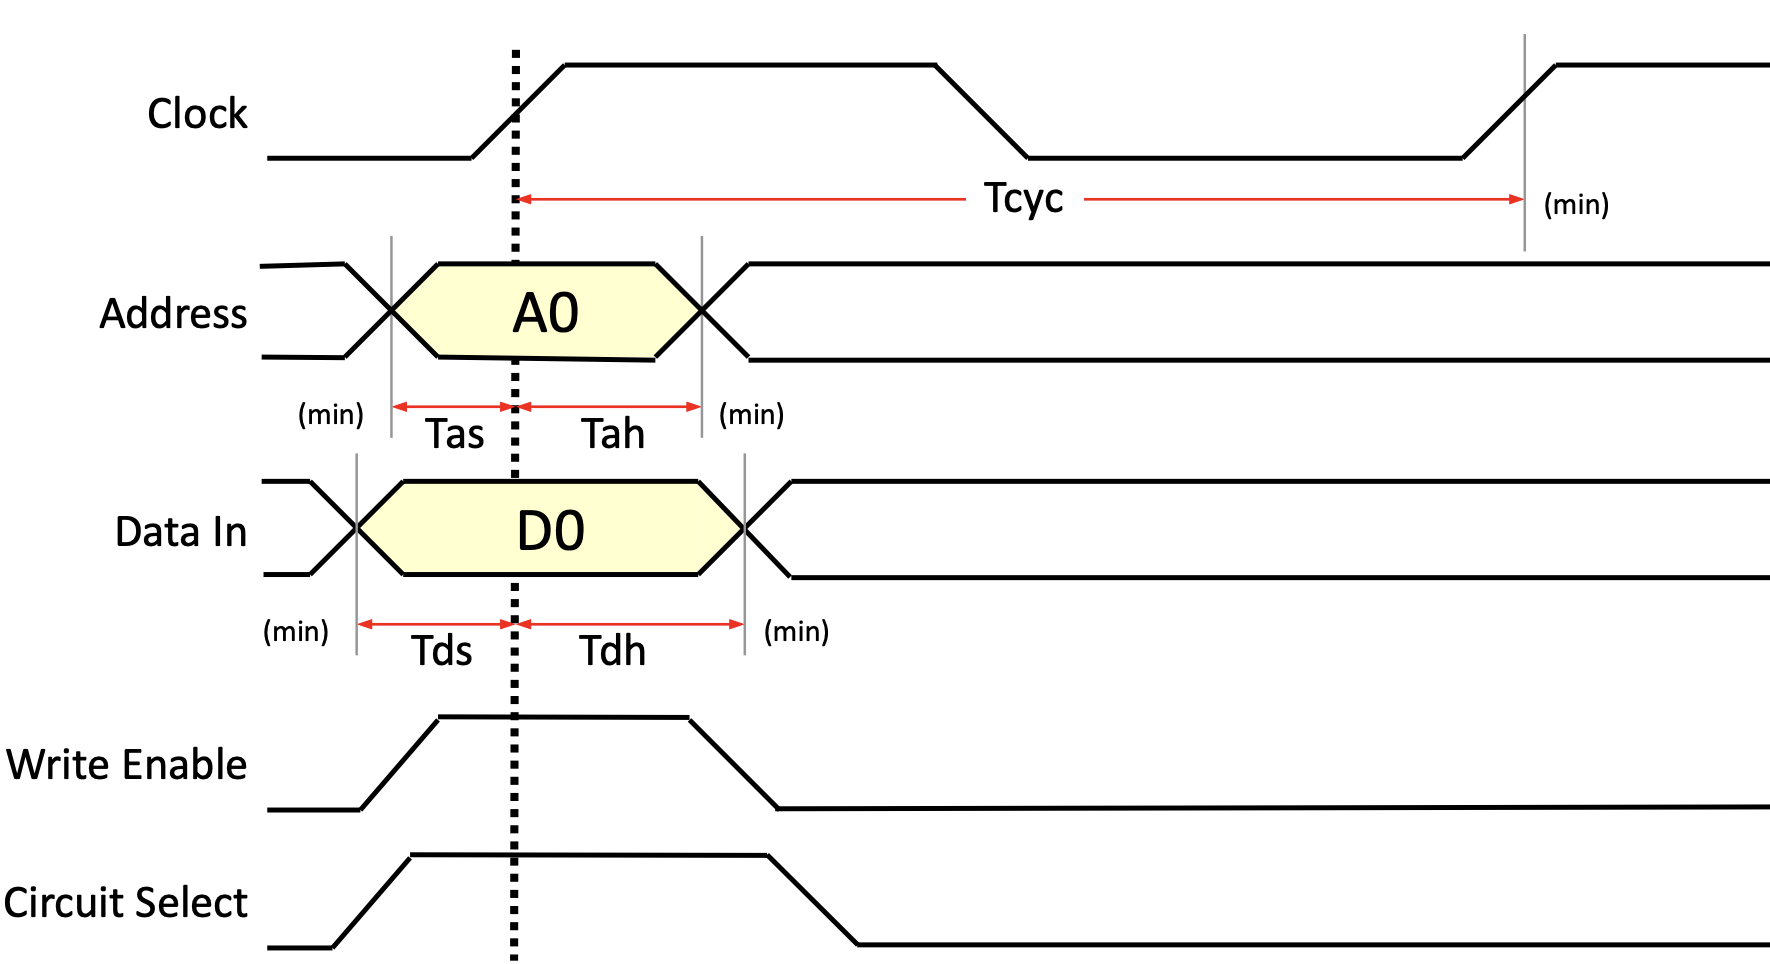
\includegraphics[width=0.45\textwidth]{chapters/chapter1c/images/write_cycle.png}
\end{center}


\section{Where is Memory in the Processor?}
\textit{In the processor we have memory in the Data memory component and in the Instruction memory component.} \\ \vspace*{5px}
\begin{center}
    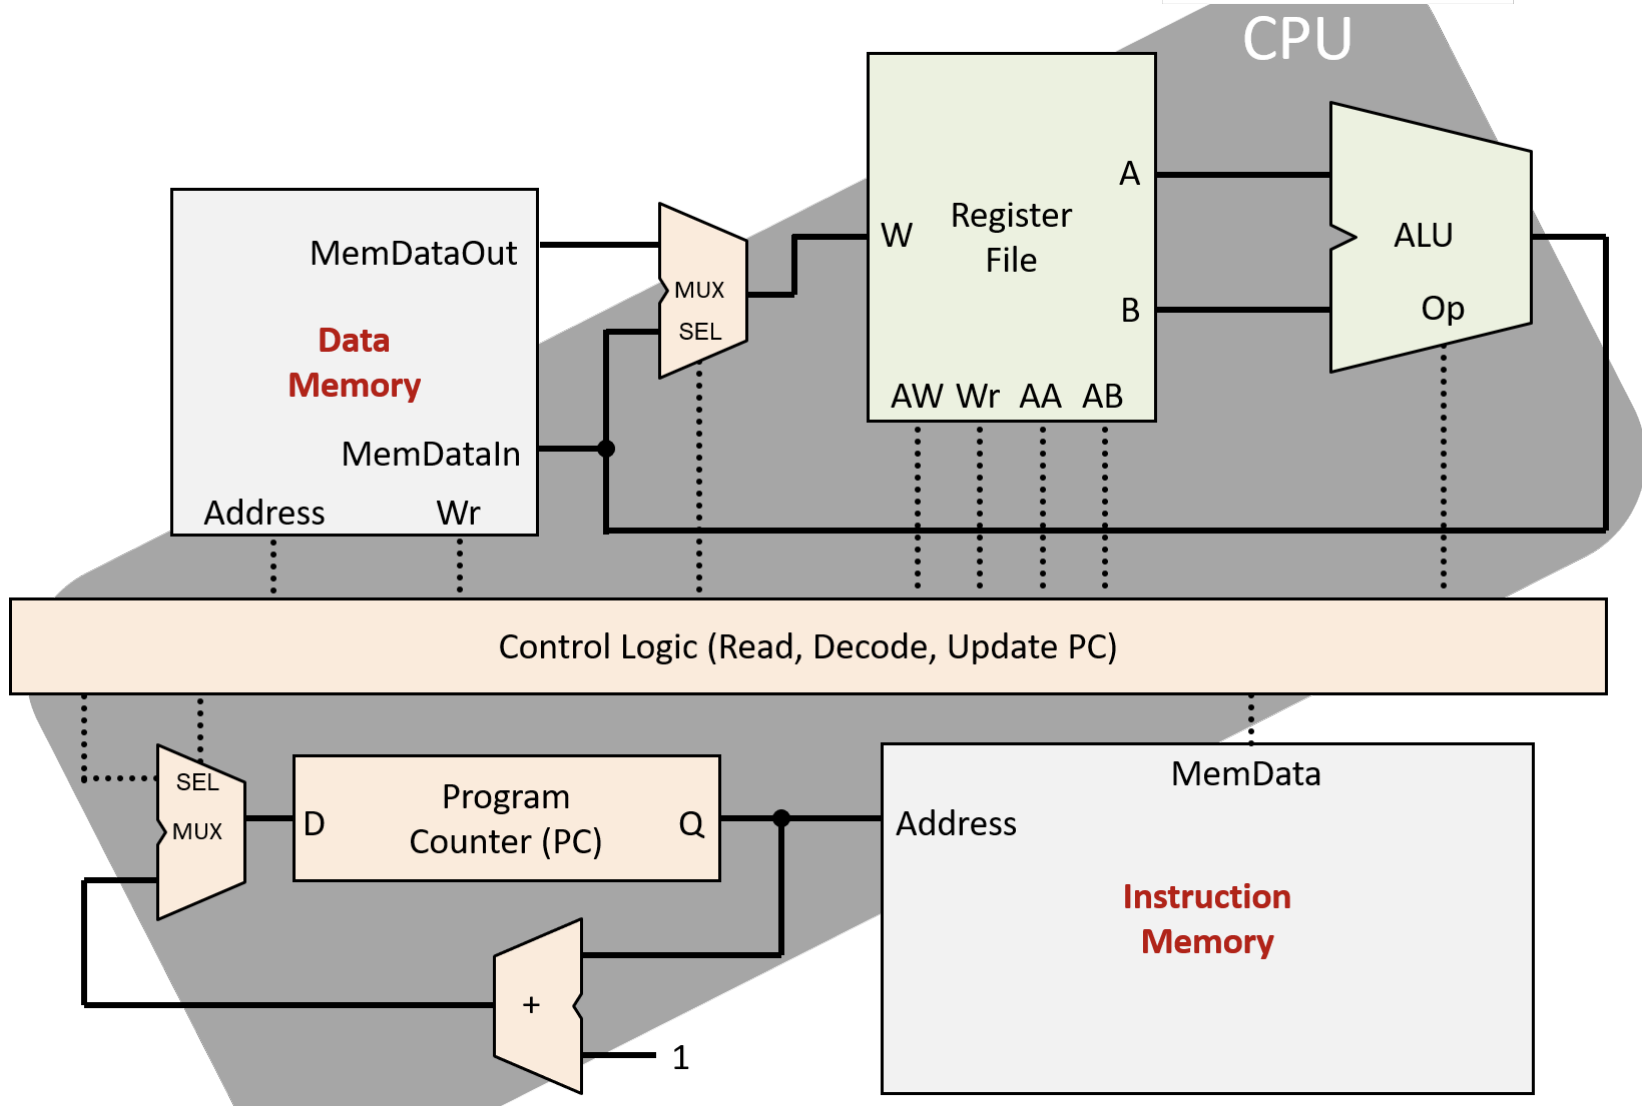
\includegraphics[width=0.45\textwidth]{chapters/chapter1c/images/processor.png}
\end{center}
\subsection{Arithmetic and Logic Instructions}
\textit{The register file can only contain a limited number of registers making it difficult to handle more complex computations and managing data input/output efficiently.}
\begin{center}
    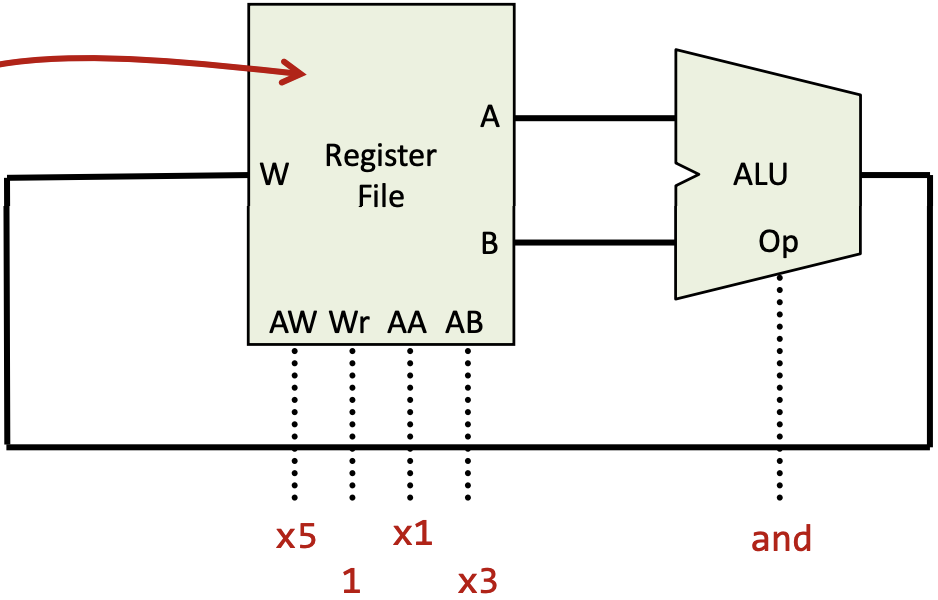
\includegraphics[width=0.45\textwidth]{chapters/chapter1c/images/arith_logic.png}
\end{center}
\subsubsection{Load Instructions}
\begin{center}
    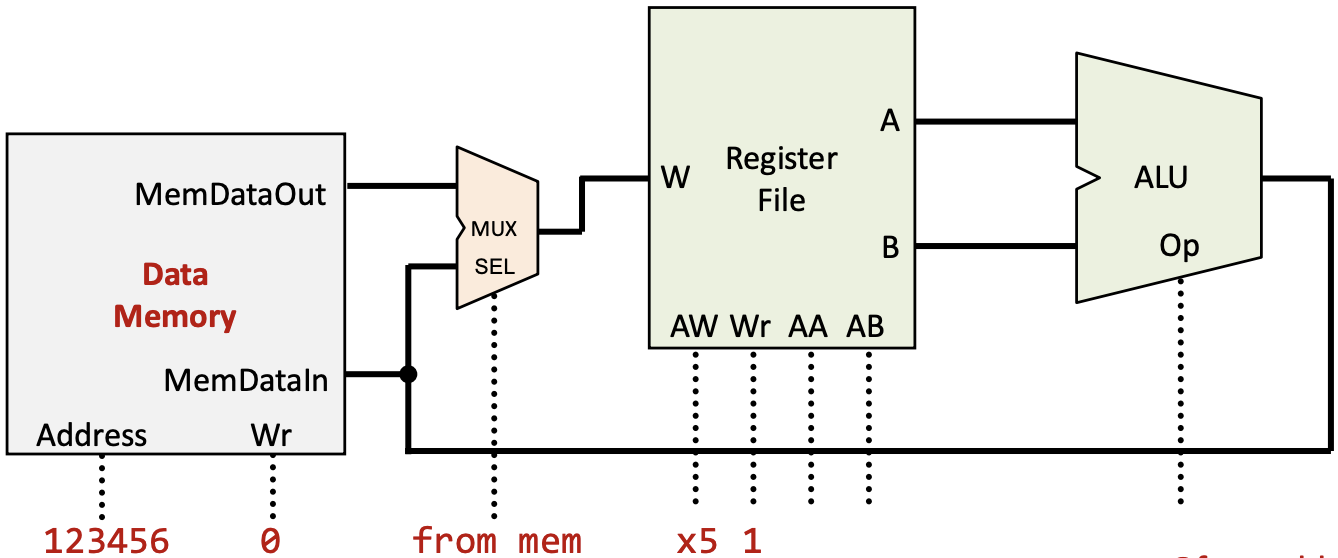
\includegraphics[width=0.45\textwidth]{chapters/chapter1c/images/load.png}
\end{center}
\subsubsection{Load and Store: The RiSC-V Way}
\textit{This instruction would never work for example because the adress is too big to be sent as an immediate value :} \texttt{lw x5, (x7)} \\ \vspace*{5px}
\begin{center}
    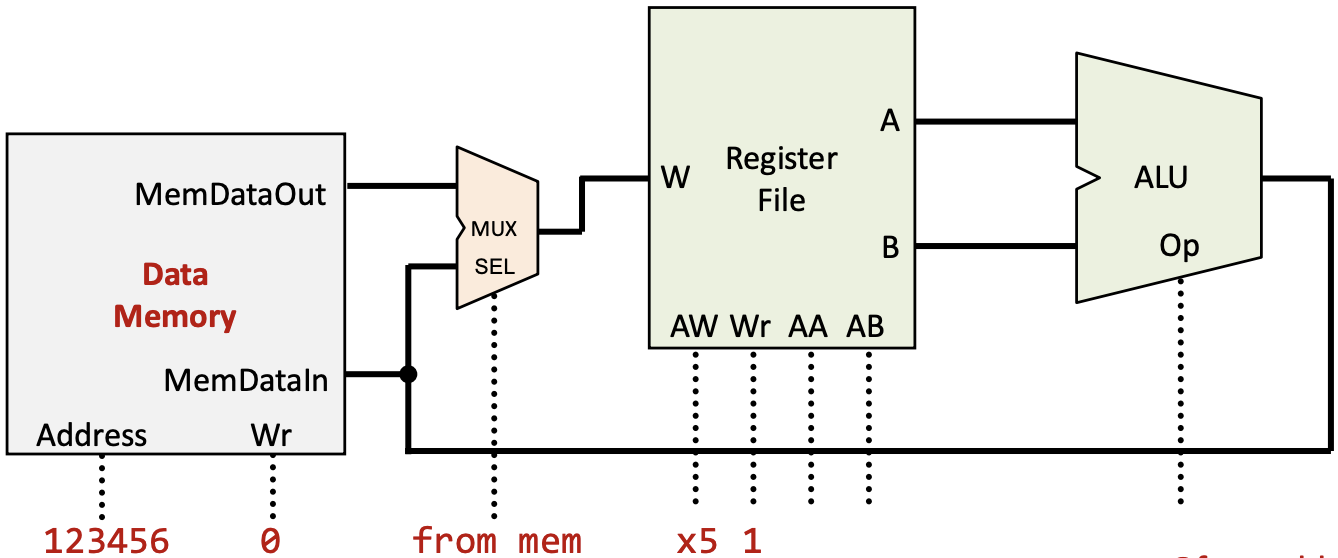
\includegraphics[width=0.45\textwidth]{chapters/chapter1c/images/load.png}
\end{center}
\subsubsection{A Load/Store Architecture}
\textit{A feature of RISC-V is that it's a Load/Store architecture, meaning that the only way to access memory is through load and store instructions. Also, instructions reading and writing in memory do exactly that and nothing else, contrary to more complex instruction set architectures (CISC), where instructions may combine memory access with other operations like arithmetic or logic. This simplicity in RISC-V's instruction set helps with streamlining the pipeline and improving performance efficiency.} \\ \vspace*{5px}

\begin{center}
    \begin{tabular}{|c|c|c|c|c|}
        \hline
        \multicolumn{2}{|c|}{\textbf{Load}} & \textbf{I} & 0x2 & 0x03 \\ 
        \hline
        \texttt{lw} & \texttt{rd,imm(rs1)} & \multicolumn{3}{c|}{\texttt{rd $\leftarrow$ mem[rs1 + sext(imm)]}} \\ 
        \hline
        \multicolumn{2}{|c|}{\textbf{Store}} & \textbf{S} & 0x2 & 0x23 \\ 
        \hline
        \texttt{sw} & \texttt{rs2,imm(rs1)} & \multicolumn{3}{c|}{\texttt{mem[rs1 + sext(imm)] $\leftarrow$ rs2}} \\ 
        \hline
    \end{tabular}
\end{center}

\section{More Addressing Modes? Not in RISC-V!}
\vspace*{-10px}
\begin{center}
\resizebox{1.1\textwidth}{!}{
\begin{tabular}{|l|l|l|}
\hline
\textbf{Addressing Mode}          & \textbf{Instruction}                                      & \textbf{Description}                                                                                   \\ \hline
\textbf{Register}                 & \texttt{add x0, x1, x2}                                   & Adds the value of \texttt{x1} and \texttt{x2}, stores the result in \texttt{x0}.                         \\ \hline
\textbf{Immediate}                & \texttt{add x0, x1, 123}                                  & Adds the value of \texttt{x1} and the immediate constant 123, stores the result in \texttt{x0}.          \\ \hline
\textbf{Direct or Absolute}       & \texttt{add x0, x1, (1234)}                               & Adds the value of \texttt{x1} and the value at memory address 1234, stores the result in \texttt{x0}.    \\ \hline
\textbf{Register Indirect}        & \texttt{add x0, x1, (x2)}                                 & Adds the value of \texttt{x1} and the value in memory at the address held in \texttt{x2}, stores in \texttt{x0}. \\ \hline
\textbf{Displacement or Relative} & \texttt{add x0, x1, 123(x2)}                              & Adds the value of \texttt{x1} and the value in memory at \texttt{x2} plus the displacement 123, stores in \texttt{x0}. \\ \hline
\textbf{Base or Indexed}          & \texttt{add x0, x1, i5(x2)}                               & Adds the value of \texttt{x1} and the value in memory at \texttt{x2} plus index \texttt{i5}, stores in \texttt{x0}. \\ \hline
\textbf{Auto-increment/-decrement} & \texttt{add x0, x1, (x2+)}                               & Adds the value of \texttt{x1} and the value in memory at the address in \texttt{x2}, then increments \texttt{x2}, stores in \texttt{x0}. \\ \hline
\textbf{PC-Relative}              & \texttt{add x0, x1, 123(pc)}                              & Adds the value of \texttt{x1} and the value in memory at \texttt{pc} plus 123, stores in \texttt{x0}.    \\ \hline
\end{tabular}}
\end{center}
    
\textit{Syntax here looks like RISC-V but most of these instructions do not exist in RISC-V.}
\newpage
\subsection{Word Adressed Memory}
\textit{In a word addressed memory, the address is the index of the word in the memory.} \\ 
\textit{The letters inside the word are identified as eg. for Hello World, H:3980, E:3981, L:3982, \dots}.
\begin{center}
    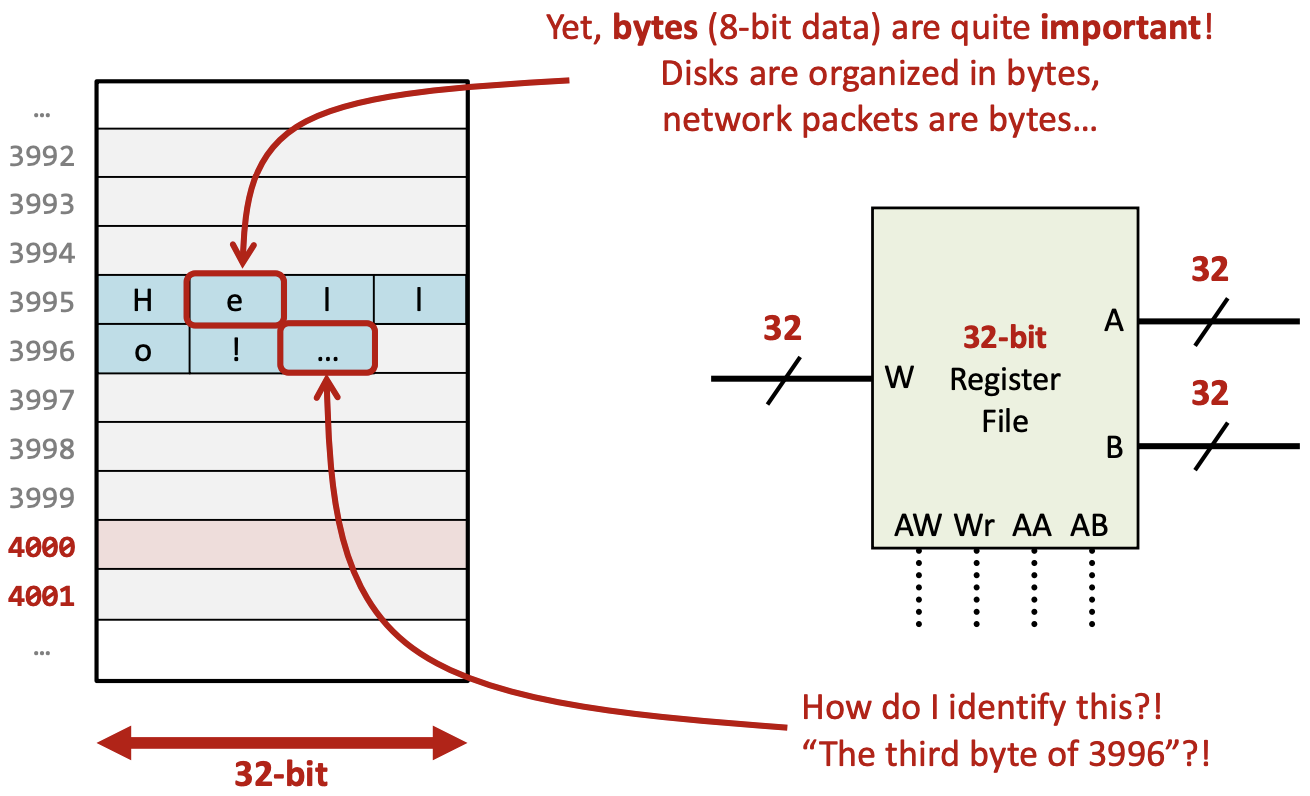
\includegraphics[width=0.45\textwidth]{chapters/chapter1c/images/word_add.png}
\end{center}

\subsection{Loading Words (lw) and Instructions}
\textit{The lw instruction is used to load a word from memory into a register.} \\ 
\textit{The adress of such words would necessarly be a multiple of 4 meaning the two least significant bits must be 0s.(to the ensure the data is word aligned\dots)} \\ 
\begin{center}
    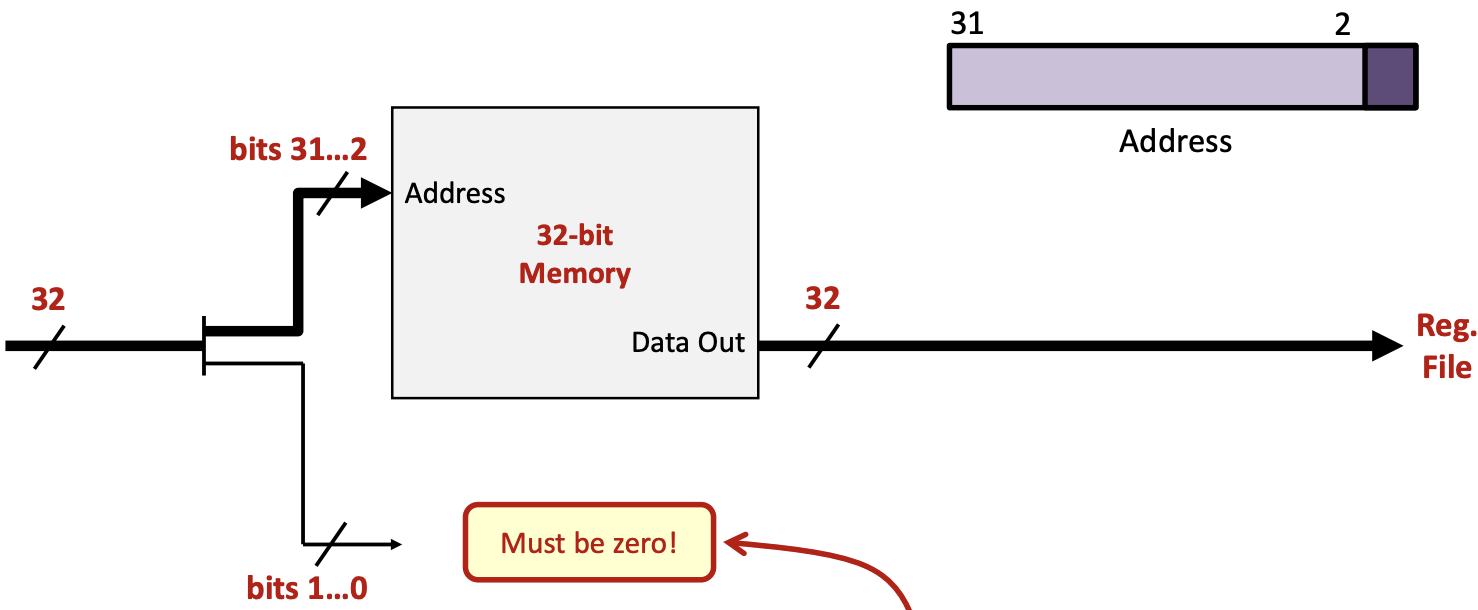
\includegraphics[width=0.45\textwidth]{chapters/chapter1c/images/lw.png}
\end{center}
\subsection{Loading Bytes (lb)}
\textit{The \texttt{lb} (Load Byte) instruction doesn't require alignment because it only loads 1 byte (8 bits), which can be accessed at any memory address, unlike \texttt{lw} which requires word alignment to efficiently load 4 bytes (32 bits).
}\textit{The lb instruction is used to load a byte from memory into a register.} \\ 

\begin{center}
    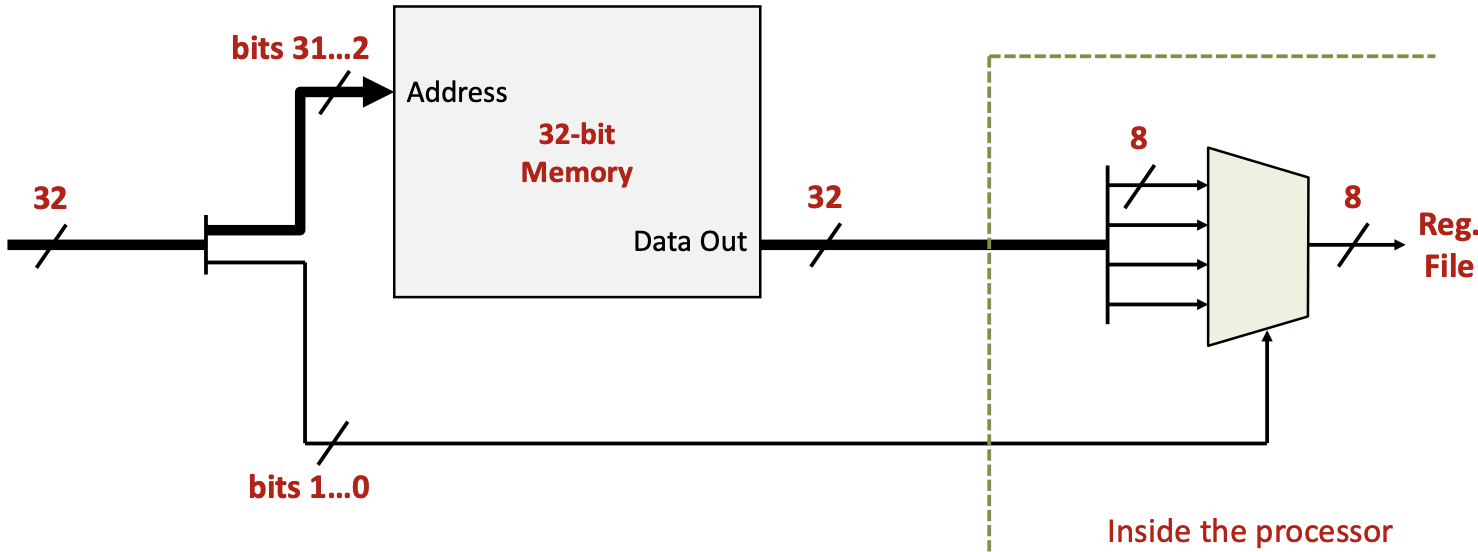
\includegraphics[width=0.45\textwidth]{chapters/chapter1c/images/lb.png}
\end{center}
\subsection{A Few More Load/Store Instructions}
\textit{Access bytes (and half-words) as if memory were made of bytes}
\begin{center}
    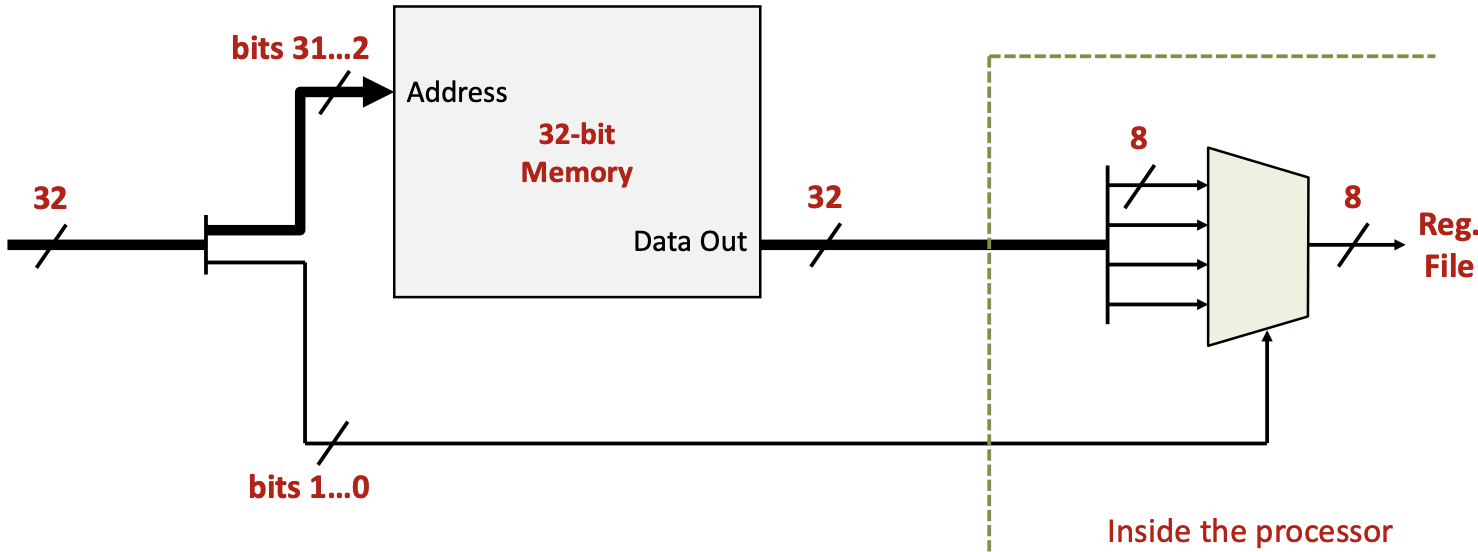
\includegraphics[width=0.45\textwidth]{chapters/chapter1c/images/lb.png}
\end{center}
\subsection{Access as it is more suitable}
\textit{For example storing the "Hello!"zero value in the memory would like this:} \\
\begin{minipage}[htp]{0.45\textwidth}
    \begin{center}
        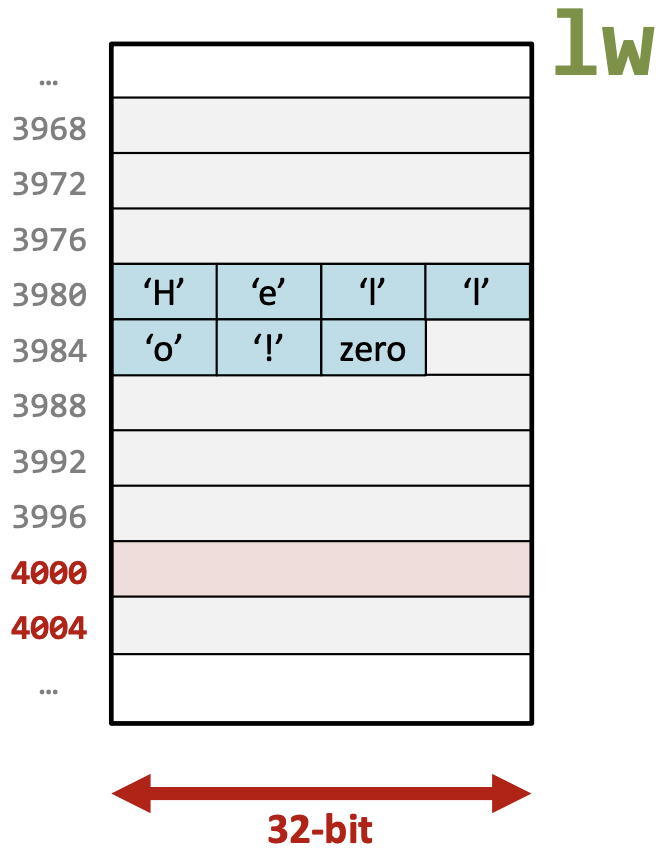
\includegraphics[width=0.45\textwidth]{chapters/chapter1c/images/hello.png}
    \end{center}
\end{minipage}
\hfill
\vline
\hfill
\begin{minipage}[htp]{ .45\textwidth}
    \begin{center}
        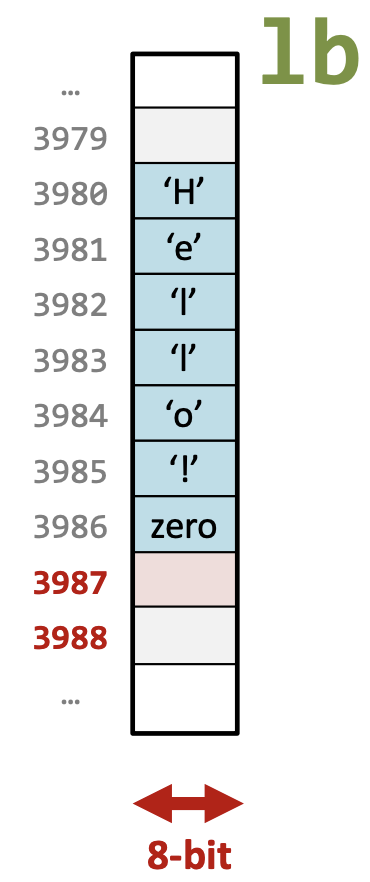
\includegraphics[width=0.3\textwidth]{chapters/chapter1c/images/hello2.png}
    \end{center}
\end{minipage}
\subsubsection{Counting Characters in a String}
\textit{As an example, for counting the number of characters in a string, the load byte instruction would be more suitable as seeing the string as a sequence of bytes makes use of the memory as a sort of array.} \\ \vspace*{5px}

\begin{center}
    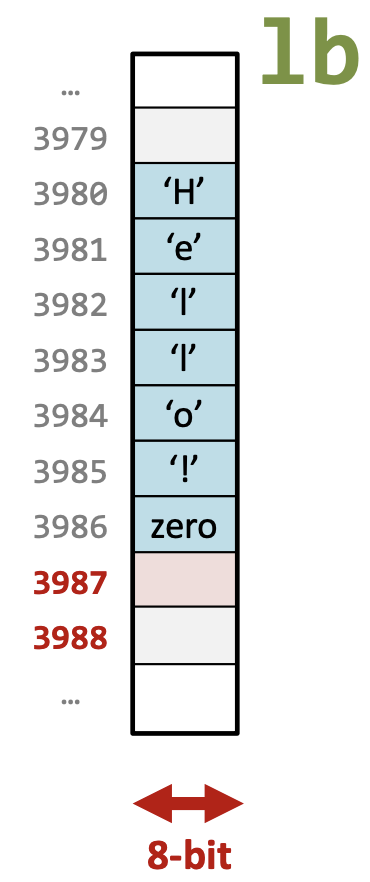
\includegraphics[width=0.15\textwidth]{chapters/chapter1c/images/hello2.png}
\end{center}
\begin{center}
    \begin{assembly}
strlen:
    mv t0, a0 # Copy the pointer (a0) into t0 to traverse the string
    li t1, 0 # t1 will hold the length (initialized to 0)
loop:
    lbu t2, 0(t0) # Load byte at address t0 into t2
    beq t2, zero, end # If t2 is 0 (null byte), we are done
    addi t1, t1, 1 # Increment the length counter (t1)
    addi t0, t0, 1 # Point to the next character in the string
j loop # Repeat the loop
end:
    mv a0, t1 # Move the length (t1) into a0 as the return value
    ret # Return to caller
    \end{assembly}
\end{center}

\textit{\texttt{lbu} is used here to ensure that the byte is treated as an unsigned value, which is the correct approach for processing characters in a string.
}
\newpage
In a word addressed memory view, the code would look like such: \\ \vspace*{5px}
\begin{center}
\begin{assembly}
strlen:
    li t1, 0           # t1 will hold the length (initialized to 0)
next_word:
    li t2, 4           # t2 will count the bytes in a loaded word (four)
    lw t3, 0(t0)       # Load four bytes at address t0 into t3
next_byte:
    andi t4, t3, 0xff  # Move the "little-end" in t4
    beq t4, zero, end  # If t4 is 0 (null byte), we are done
    addi t1, t1, 1     # Increment the length counter (t1)
    srli t3, t3, 8     # Prepare the next byte of the word in the "little-end" (t3)
    addi t2, t2, -1    # One byte left in the loaded word
    bnez t2, next_byte # If more bytes in t3, check the next
    addi a0, a0, 4     # Else point to the next word of characters in the string
    j next_word        # Repeat the loop
end:
    mv a0, t1          # Move the length (t1) into a0 as the return value
    ret                # Return to caller
\end{assembly}
\end{center}
\subsection{Loading Bytes (lb)}
\textit{Now, one may wonder in what ordering the bytes are stored in memory.} \\ \vspace*{5px}
\begin{center}
    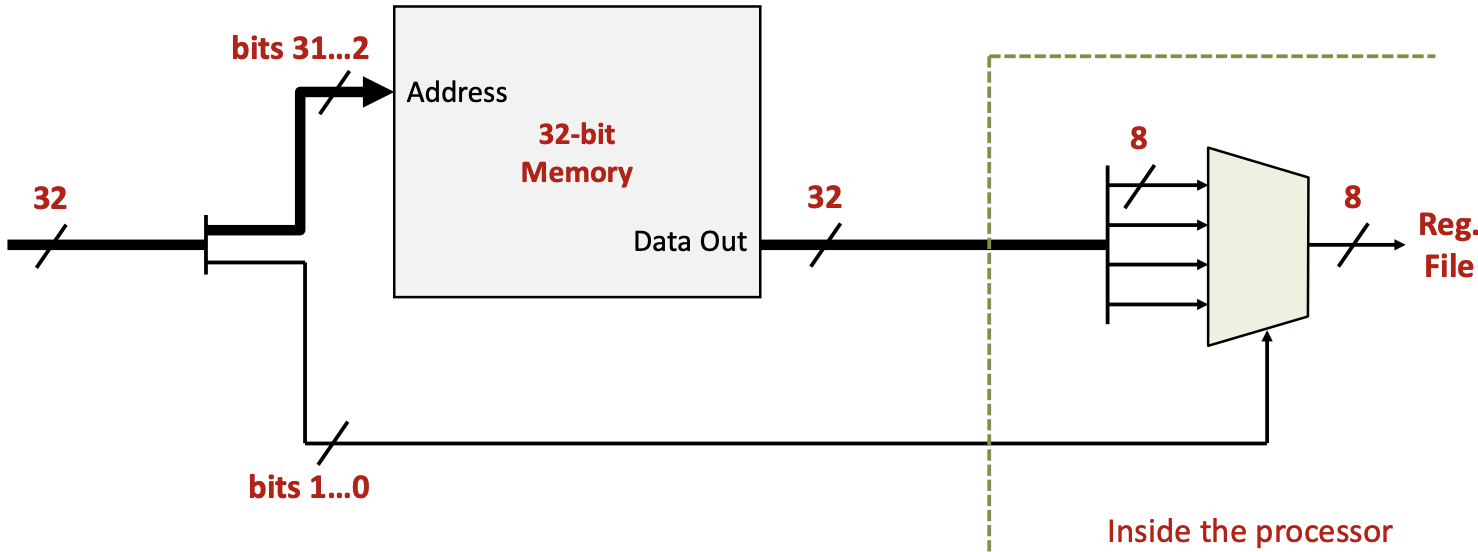
\includegraphics[width=0.55\textwidth]{chapters/chapter1c/images/lb.png}
\end{center}
\subsubsection{Which Byte Where?}
\textit{Both ordering of bytes are valid the only thing we have to do is stick to one, the most generally used is little-endian as it's the RISCV default and the Intel x86/x64 default.} \\ \vspace*{5px}
\begin{minipage}[htp]{0.45\textwidth}
    \begin{center}
        \textbf{Little Endian} \\ \vspace*{5px}
        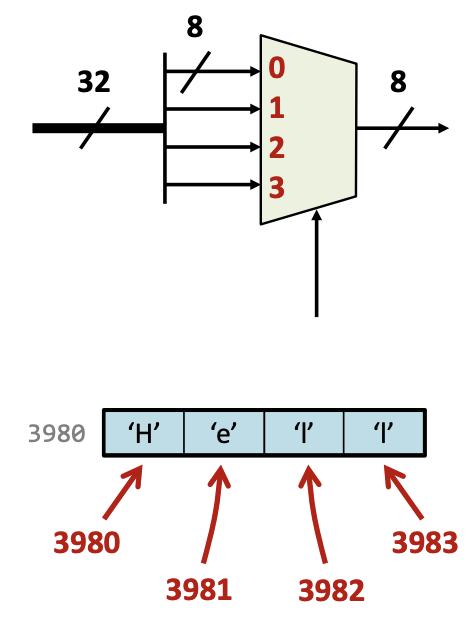
\includegraphics[width=0.55\textwidth]{chapters/chapter1c/images/bytes.png}
    \end{center}   
\end{minipage}
\hfill
\vline
\hfill
\begin{minipage}[htp]{0.45\textwidth}
    \begin{center}
        \textbf{Big Endian} \\ \vspace*{5px}
        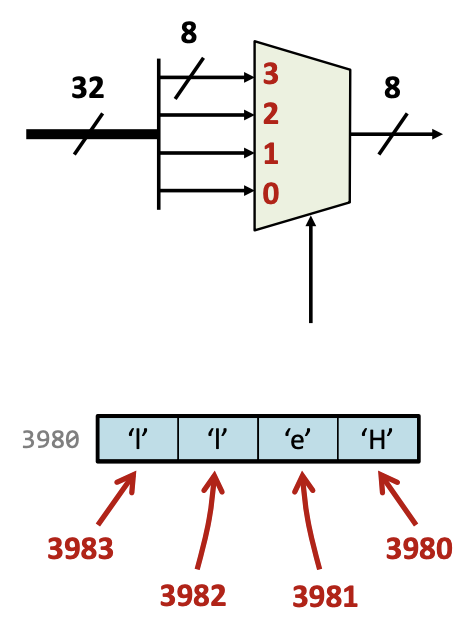
\includegraphics[width=0.55\textwidth]{chapters/chapter1c/images/bytes2.png}
\end{center}
\end{minipage} \\ \vspace*{5px}
\textit{Personal Remark : Mnemotechnic - Little Endian = Little End (The ending memory index takes the smallest(starting) data adress), Big Endian = Big End.}